%% LyX 2.3.1 created this file.  For more info, see http://www.lyx.org/.
%% Do not edit unless you really know what you are doing.
\documentclass[english]{article}
\usepackage[T1]{fontenc}
\usepackage[latin9]{inputenc}
\usepackage{amsmath}
\usepackage{amssymb}
\usepackage{graphicx}

\makeatletter

%%%%%%%%%%%%%%%%%%%%%%%%%%%%%% LyX specific LaTeX commands.
%% Because html converters don't know tabularnewline
\providecommand{\tabularnewline}{\\}

\makeatother

\usepackage{babel}
\begin{document}
\title{A Semi-Markov Approach to Study a Group of Kinesin Motors}
\maketitle
\begin{abstract}
We propose a general approach to study cellular transport by a group
of kinesin motors. Our approach can integrate kinetic models of a
single kinesin motor, including detachment and reattachment events, to study the group behaviors of several motors. By formulating the problem as a semi-Markov process and applying a central limit theorem, asymptotic velocity and diffusivity can be readily calculated, rendering considerable computational advantage over Monte Carlo simulations in tasks such as parameter sensitivity analysis and model selection. We demonstrate the method with some examples and point out the importance of capturing the intrinsic microscopic-level dynamics of individual motors and how changes at the microscopic level propagate to the motor-cargo at a mesoscopic level. 
\end{abstract}

\section{Introduction}

Intracellular transport is vital for the proper functioning of a biological cell. Passive diffusion is inadequate for long-distance transport of large cellular cargo, such as vesicles and organelles. Eukaryotic cells evolved an active transport system involving motor proteins which move on a track called microtubules (MTs) towing cargo to needed locations. Kinesin is one such motor protein. A kinesin has two motor domains, typically called heads, which can bind both ATP and the MT (cite some stuff). By utilizing the energy from ATP hydrolysis, a kinesin ``walks'' on the MT towards the plus end using its two heads in a hand-over-hand fashion, undergoing a sequence of tightly coupled mechano-chemical transitions. Many studies have been conducted on single motors and given us a good understanding of its function in isolation{[}{]}. The sequence of mechano-chemical transitions are described by kinetic models and are often formulated as a continuous-time Markov chain\cite{Clancy2011}. It is known that at least some of the transition rates are force dependent{[}{]}. 

In cellular environments, molecular motors work in a group to transport cargo{[}{]}. Motors are linked to a common cargo by a flexible polymer, forming a motor-cargo complex. When motors in the group drift apart, tension is built up between them; this tension is resolved by either detachment-reattachment or force-induced changes in the stepping rates of individual motors. In this sense, their motion is coupled together through the cargo, and keeping the complex together. When opposing motors are attached to a single cargo, intriguing bidirectional movements may be observed which have triggered substantial interest in studying transport of multiple coupled motors\cite{Hancock2014}. Although there have been many experimental and theoretical studies, how our understanding of a single motor can inform their behaviors in a motor-cargo complex remains unclear. 

Stochastic modeling has a fruitful history in generating insight in
cellular transport \cite{Bressloff2013}. In previous modeling studies on multiple motors, the details of underlying kinetics of individual motors and how the cargo load is shared between them have often been overlooked \cite{Miles2018a,McKinley2012,Ohashi2019}. In this work, we propose an approach to study a group of molecular motors which takes into account microscopic details of individual motors. We treat loading forces shared between motors by making them dependent on motors' relative positions. We focus on kinesin since its molecular mechanisms are better understood, allowing us to incorporate existing kinetic models into the framework we will present. By formulating semi-Markov process and invoking a functional CLT, asymptotic quantities for the position of the motor-cargo complex can be easily calculated by a few computationally modest matrix operations. 

The paper is outlined as follows. We first describe the semi-Markov approach in general.  Then, we show how this framework can be applied to motor-cargo complexes. Taking advantage of its computational efficiency, we then conduct a study of the system with a wide range of parameter choices. 

\section{Semi-Markov Framework for Molecular Motor Models}

In this section, we present a previously established framework for molecular motor models that break each kinetic cycle into a time and a displacement (cite my stuff and others) and then to use central limit theory to establish asymptotic quantities typically measured in experiments.  The goal of this paper is to generalize the technique to motor-carg complexes.

We consider a Markov chain $\{S_{i}\}_{i\in\mathbb{N}}$ where $S_{i}$
represents the relative position and the kinetic state (together called the
``group state'' henceforth) of each motor at ``time'' $i$. We
adopt an underlying kinetic model for each motor which governs how
the motor transitions through biochemical states. Note that every time
a motor changes its kinetic state, the group state changes while the
relative position only changes if the motor makes a transition which
results in a physical step. Let $\tau_{i}$ be the time for the transition
of $S_{i}\to S_{i+1}$ to happen and $Z_{i}$ be the change in the
group position (arithmetic average of positions of all motors) resulting
from this transition. If we assume the transition from $S_{i}\to S_{i+1}$ follows
every change in the group state due to a transition in the underlying
kinetic states of individual motors, then $\tau_{i}$ is a exponential
random variable. {\bf JF: I don't quite understand the following two sentences.}  In general, neither the state space of $\{S_{i}\}$
needs to the set of all possible group states and nor does the transition
of $S_{i}\to S_{i+1}$ to exactly follow every change in the group
state due to the individual motors' kinetic transitions. Being aware
of this sometimes would help simplify calculation as we will see later. 
{\bf JF: I think you need to explain the dependency between the S, Z, and tau in words--specifically that they form a three dimensional Markov chain--where Z, tau at the current time depend only on S at the previous time.}

Let $X(t)$ be the group position at time $t$. Using the variables
defined above, we can write $X(t)=\sum_{i=1}^{N(t)}Z_{i}$ where $N(t)=\inf\{n\in\mathbb{N}:\sum_{i=1}^{n}\tau_{i}\ge t\}$.
Two quantities commonly observed in experiments and studied theoretically
are asymptotic speed and diffusivity, i.e., $V=\lim_{t\to\infty}\frac{E[X(t)]}{t}$
and $D=\lim_{t\to\infty}\frac{\text{Var}[X(t)]}{2t}$. Since experimental
observations of motors occur at significantly long time and distance
in contrast to microscopic motor dynamics, from a CLT (central limit theory) point of view,
we are looking effectively at a Brownian motion. To make it precise,
we want to cast a multiple-motor model into a framework of semi-Markov
processes so that these two asymptotic quantities of interests can be
easily calculated using a functional CLT. Towards this goal, we consider
a discrete-time Markov chain 
\[
\begin{pmatrix}Z_{i}\\
\tau_{i}\\
S_{i}
\end{pmatrix}
\]
for which we impose the following assumptions:
\begin{enumerate}
\item $S_{i}$ has a stationary distribution on a finite state space and
is aperiodic. 
\item conditioned on a sequence $\{S_{i}\}_{i\in\mathbb{N}}$, the sequence
$\{(Z_{i},\tau_{i})\}_{i\in\mathbb{N}}$ are independent.
\item $\{(Z_i, \tau_i, S_i)'\}$ is a Markov chain whose distribution at time $i$ conditioned on the chain at $i-1$ depends only on $S_{i-1}$.
\item $P(Z_{i}\vert\{S_{j}\}_{j\in\mathbb{N}})=P(Z_{i}\vert S_{i})$ and
$P(\tau_{i}\vert\{S_{j}\}_{j\in\mathbb{N}})=P(\tau_{i}\vert S_{i})$ 
\item first two moments of $Z_{i}\vert S_{i}$ and $\tau_{i}\vert S_{i}$
are finite and known
\end{enumerate}
Scaling time with a factor $n$ and length by $\sqrt{n},$ we have by functional
CLT 
\[
\sqrt{n}\big(X(nt)-Vnt\big)\Rightarrow\sqrt{2D}B(t)
\]
as $n\to\infty$ where $B(t)$ is standard Brownian motion. The asymptotic
quantities can be calculated using a modified functional CLT (see
derivation in \cite{Hughes2011}) so that we have
\begin{equation}
V=\lim_{t\to\infty}\frac{E[X(t)]}{t}=\frac{\mu_{z}}{\mu_{\tau}}\label{eq:V}
\end{equation}
 and 
\begin{equation}
D=\lim_{t\to\infty}\frac{\text{Var}(X(t))}{2t}=\frac{1}{2}(\frac{\mu_{Z}^{2}\sigma_{\tau}^{2}}{\mu_{\tau}^{3}}+\frac{\sigma_{Z}^{2}}{\mu_{\tau}}-2\frac{\mu_{Z}\sigma_{Z,\tau}}{\mu_{\tau}^{2}})\label{eq:D}
\end{equation}
where $\mu_{i}$ and $\sigma_{i}^{2}$ are mean and variance of $i\in\{Z,\tau\}$,
and $\sigma_{Z,\tau}$ denotes covariance of $Z$ and $\tau$. {\bf I'm not crazy about this $\mu_{i}$ notation.} The
application of a functional CLT in obtaining asymptotic quantities in studying
molecular motors dated back to \cite{Hughes2011,Krishnan2011} and semi-Markov
processes were introduced in \cite{Hughes2012} to study variable
step sizes.{\bf JF: you may also want too cite Arjun Krishnan here.  Also, maybe look for other people's similar approaches to multiple motors.} Here we extend this method to a group of motors. We can
find $\mu_{i}$ and $\sigma_{i}$ by finding the moments conditioned on the stationary distribution of $S_{i}$(details summarized in the appendix).

\subsection{Two Examples }

We illustrate the use of the semi-Markov approach by applying it to two
kinetic models. First, we state the common modeling assumptions. Let
$m$ be the number of motors linked by a linear spring with constant
$k_{i}$ to a common cargo which equilibriates instantaneously. It
should be noted that the cargo is modeled as not having Brownian forces
acting on it---which is not really the case---but also not an unreasonable assumption---effectively
we are averaging a fast cargo. Similar approximation has been made in \cite{Peskin2000,Fricks2006,McKinley2012} {\bf JF: Cite multipaper with Pete, Scott, etc  Also, Elston}. Each of the motors walks on a MT without
direct interactions with others, i.e., the only coupling is via the
common cargo. Motors can detach and reattach to the MT. Motors share
the loading force $F$ by force balance 
\[
F=\sum_{j=1}^{m}k_{j}x_{j},
\]
where $x_{i}$ are the displacements of the spring connecting to the
i-th motor ($x_{i}>0$ for displacements in the hindering direction
and $x_{i}<0$ vice versa). Hence the loading force felt by the i-th
motor is $k_{i}x_{i}.$ In this modeling framework, the state $S_{i}$
consisting of 
\begin{itemize}
\item relative positions of $m$ motors (Here we take it exactly as $\{x_{i}\}_{i\in1...m}$
though some slack regime possibly exists. {\bf JF: what does slack regime mean} ) 
\item their kinetic states (including detachment as a state). 
\end{itemize}
Moreover, in the kinetic model we wish to adopt, at least one of the
transitions is force-dependent and its rate is thus affected by which motors are coupled to that motor. In the following, we present details on how to apply this approach through some examples. 

\subsubsection{A Standard 3-state Motor Model}

We consider a standard 3-state model of a single kinesin stepping\cite{Andreasson2015}
\[
\begin{array}{ccccccc}
 & E\\
\swarrow &  & \nwarrow\\
A & \rightleftharpoons & B & \to & C & \to & A(+1)
\end{array}
\]
where $A$ represents the state of one head bound and the other awaiting
for ATP binding, $B$ represents ATP bound state, $C$ is two heads
bound state and $E$ is the detached state. For simplicity, we only
include forward stepping. Transition $B\to C$ represents the configuration
change where the unbound head docks and attach to the binding site.
So it is reasonable to make this step force dependent, where we assume
a Bell's law dependence. 

We assume there are two motors in a group for simplicity. In this
case, $S_{i}=(x_{1}-x_{2},K_{1},K_{2})$ where $K_{1},K_{2}$ are the chemical states of motors 1 and 2 and take values in the set $\{A,B,C,E\}$.
$S_{i}$ transitions to $S_{i+1}$ every time one of the motor makes
a kinetic transition. We can verify that $S_{i}$ satisfies the assumptions
we imposed earlier.

In theory, since motors can be any number of binding sites away from
each other, the state space of $S_{i}$ is infinite, which is not
ideal for computer implementation. In reality, the polymer (say DNA
links in DNA orgami experiment) that connects to the motor, though
flexible, should have a contour length that limits how far motors
can be separated. In our implementation, since the contour length
information is not available, we adopt another strategy to restrict
state space be finite. We note that unrealistic far separation are
rare and hence including them would only make negligible differences
in our results. Therefore, we gradually increase the number of possible
configurations from close to far until changes in the calculated asymptotic
results are tiny. In this way, $S_{i}$ has a finite state space and
its transition matrix can be formed. Moreover it is irreducible and
hence it has a unique stationary distribution. Aperiodicity is easily
seen by tracking the number steps back to certain state. {\bf JF: not sure about this last sentence--don't quite follow.}

Assumption 2 is basically the semi-Markov property which states that the
next transition only depends on the current state but does not depend
on previous states. 

Assumption 3 is also readily verified. First we note that $\tau_{i}\vert\{S_{j}\}_{j\in\mathbb{N}}=\tau_{i}\vert S_{i}\sim Exp(\text{\ensuremath{\lambda}})$
where rate $\lambda$ is the sum of rates of all transitions out of
$S_{i}$. Also, $Z_{i}\vert\{S_{j}\}_{j\in\mathbb{N}}=Z_{i}\vert S_{i}$
is 0 if $S_{i}$ has no motors in state $C$ and 1/2 otherwise. 

\subsubsection{A More Complex Model with Quasi-stationary Approximation}

One drawback of our semi-Markov approach is that the number of states
grows factorially with number of motors. In experimental studies such as the DNA origami experiments described in the introduction,
only a few motors are involved. So it is less a concern when modeling
those situations. Moreover we can make a quasi-stationary approximation
to further mitigate the issue. In this case, consider a 4-state kinetic
cycle (e.g. the one in \cite{Hughes2011}) 
\[
\begin{array}{cccccc}
 &  & \swarrow\nearrow & A & \leftrightarrow & B\\
 & E &  & \updownarrow &  & \updownarrow\\
 &  & \nwarrow\searrow & F & \leftrightarrow & C
\end{array}
\]
where $E$ is detached state. In this case, completing a clockwise
cycle means a forward step and vice versa for backward stepping. Although
the end (or start) of a cycle can be arbitrary appointed, we have
to be careful in order to use a quasi-stationary approximation. To
make a quasi-stationary argument, we need to identify the rate limiting
transition in the cycle. Say transitions $A\rightleftharpoons F$
is much slower than other transitions then we can think the cycle
as follows 
\[
F(-1)\leftarrow A\rightleftharpoons B\rightleftharpoons C\rightleftharpoons F\rightarrow A(+1)
\]
where we count a forward step whenever transition $F\rightarrow A$
occurs and a backward step whenever transition $A\to F$ occurs. We
only track the kinetic state of the motor that just made a step and
assume that all other motors are in a stationary distribution of $A\rightleftharpoons B\rightleftharpoons C\rightleftharpoons F$.
The number of kinetic states of a $m-$motor system is $2m$, (e.g.
for two motors we have $AS,FS,SA,SF$ where $S$ represents ``stationary
state''. We call this approximation ``qss2''. It drastically reduces
the state space. However it can be seen that the third assumption
is not met, i.e., $P(Z_{i}\vert\{S_{j}\}_{j\in\mathbb{N}})=P(Z_{i}\vert\{S_{i},S_{i+1}\})\neq P(Z_{j}\vert S_{j})$
(same for $\tau$). For example, if $S_{i}=0AS$, there are four possible
$S_{i+1},$ i.e., $1AS,-1FS,-1SA,1SF$, conditioned on which we have
$Z_{i}=+1,-1,+1,-1$ respectively. It should be pointed out that this
issue arises more generally when the stepping is not the only possible
transition for the pre-stepping states. The way around this issue
is to consider the ``augmented chain'' $\{(S_{i},S_{i+1})\}_{i\in\mathbb{N}}$
in which transitions of the original chain are now states. In this
way, $Z_{j}|(S_{j},S_{j+1})$ is deterministic and distribution $p(\tau_{j}|(S_{j},S_{j+1}))$
is not exponential anymore but it can be found using the matrix computational
method in \cite{Hughes2011}. Moreover, the state space can be further
reduced if all motors are identical. Taking one step further, if we
assume that the mixing time is negligible, i.e., the newly stepped
motor get into stationary distribution instantaneously, then there
is no need to track the kinetic state of motors any more so that the
method can easily handle up to five motors . We call this approximation
``qss1''. 

\section{Modeling experiments}

In this section, we conduct in silicon experiments to study various
behaviors of the two models we introduced previously. This extensive
study is made possible thanks to the flexibility and efficiency of
the semi-Markov approach. 

\subsection{standard 3-state model}

For this model, we consider a 2-motor system for simplicity. We adapt
biological relevant parameters found in literature shown in table\ref{tab:parameters}.
In Fig\ref{fig:FV 1-2-motor}, the single-motor kinetic model gives
a force-velocity curve of a typical sigmoid shape. It can be seen
that the motor is insensitive to small hindering (positive) force
and that the assisting (negative) force only speeds up the motor slightly.
It indicates that there are two regimes: one is force-dependent transitions
being rate-limiting while the other is limited by force-independent
transitions. The diffusivity curve has a similar shape. We found that
a 2-motor system is in general slower than 1-motor system when operated
under assisting or small hindering force, which agrees with previous
studies\cite{McKinley2012}. This indicates that two motors tend to
interfere with each other. This is expected considering the characteristics
of the single-motor force-velocity relation, i.e., the leading motor
would be slowed down by the drag caused by the lagging motor while
the dragging motor would not speed up because of the assistance from
the leading motor. However, when the 2-motor system is under heavy
load, they tend to share the load and can go faster than 1-motor system.
We call the force at which the force-velocity curve of the 2-motor
system intersects with that of the 1-motor system the ``compensation
force''. Beyond compensation force, the multiple-motor system is
faster than the 1-motor system. It is an interesting quantity to study
since it may have something to do with optimality of the cell, i.e.,
how many motors is optimal to transport certain size of cargo. We
also note that including detachment in the 2-motor model makes some
qualitative change in the force velocity curve. The monotonicity of
the force-velocity is lost: it dips down at high assisting force.
It is likely due to the fact that 2-motor system tend to have more
frequent detachment under large force. Since detachment plays an important
role, we consider the model with detachment henceforth. 

Second moment is less often studied in experimental studies. In Fig\ref{fig:M2},
we show an example in which difference in second moment of the single
motor behavior can give arise salient differences in the first moment
of the group behavior. As we can see, the first parameter set(kab=500)
gives monotonic force-velocity curve while we lose monotonicity for
the second parameter set (kab=5000). So the in first parameter set,
force-dependent transition is the dominant rate-limiting step for
the range of force we considered while in the second parameter set
other transitions is rate-limiting when assistance force is large.
In general, we see that the loading force decreases diffusivity and
that the diffusivities of 1-motor and 2-motor systems tend to converge
at large loading force. It should also be noted that force-velocity
curve alone is not sufficient to idnefity all parameters of such a
simple kinetic model. To avoid unidentifiability, care should be given
in parameter fitting and model formulation. 

Next, we conduct sensitivity analysis for compensation force. We focus
on reattachment rate since its information is scarce in literature.
We hope our theoretical study will stimulate experimental studies
on this front. We also want to find out effects of asymmetry in detachment
in response to the assisting and hindering force on compensation.
We suspect that favorable detachment under assisting load can result
in increase in velocity. As in Fig\ref{fig:fcomp surf}, our results
show that asymmetry in detachment rate plays only a marginal role
when using reported kinesin detachment rate. It asserts more influence
on compensation force when we use large detachment rate. It should
be noted that detachment only happens at state A in our model. Thus
the $k_{det}$ in our model is a different rate from most reported
detachment rates which are first order averages. In addition, we notice
that increasing $\delta_{4}$ only decrease compensation force when
reattachment is fast. However, when reattachment is slow, front motor
detachment tends to slow down the system since the system more often
operates with only one engaged motor. (want a regime where asymmetric
detachment helps only when katt is large enough (katt=200,kdet=40
both needs be large)!!

Moreover our framework easily generates stationary distribution of
motor configurations (proportion of time the system stays in each
configuration). In Fig \ref{fig:stationary-distribution}, we see
that the distribution is symmetric and centered at zero when two motors
are identical. The symmetry is not a surprise since two motors are
identical. Furthermore, We test the case of a group of two motors
of different types by selecting two parameter sets representing kinesin1
and kinesin2. We find that the distribution skewed to the left indicating
that kinesin1 tends to be ahead of kinesin2. In both cases, variance
of the stationary distribution decreases with loading force. 

By adding zero-attached-motor state as a absorbing state, we can calculate
the expected run length. In Fig\label{By-adding-zero-attached-motor},
we notice the force-run length curves are not symmetric, which is
likely due to asymmetric force-velocity response to assisting/hindering
force. However run length decreases faster with assisting force. It
is possibly due to the large variance of distribution of configuration
under assisting force, i.e., the motor explore the configurations
space more extensive increasing the exposure to more vulnerable situations
that leads to detachment. In general, we observe that run length is
very sensitive to change in $k_{det}$. 


\begin{figure}
\centerline{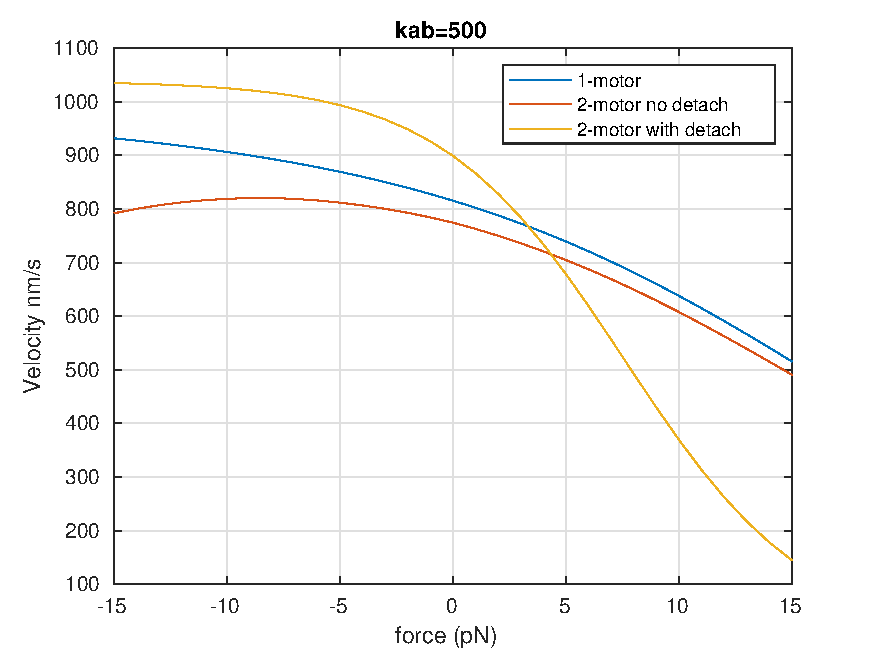
\includegraphics[scale=0.5]{figures/abc/1-2-w-wo-detach/FV-kab500}}
\caption{\label{fig:FV 1-2-motor}force-velocity curves of a single motor,
2-motor complex with and without detachment}
\end{figure}

\begin{figure}
\centerline{\includegraphics[scale=0.55]{\string"figures/abc/500vs5000 new/new/500vs5000\string".pdf}}

\caption{\label{fig:M2}force-velocity, force-diffusivity and force-coefficient
of variation curves of single motor and 2-motor complex in two parameter
sets. Note that second moment of the single motor has effects on the
first moment of 2-motor complex.}

\end{figure}
\begin{figure}
\includegraphics[scale=0.5]{\string"figures/abc/fcomp vs katt and delta/fcomp vs katt and delta\string"}\includegraphics[scale=0.5]{\string"figures/abc/fcomp vs katt and delta, kdet5/fcomp vs katt and delta\string"}



\caption{\label{fig:fcomp surf}surface plot of compensation force vs $k_{att}$
and $\delta_{4}$}

\end{figure}
\begin{figure}
\includegraphics[scale=0.5]{\string"figures/abc/xs std bar plot/xs std bar plot\string".pdf}\includegraphics[scale=0.5]{\string"figures/abc/kin1-kin2/stdistr xs\string".pdf}

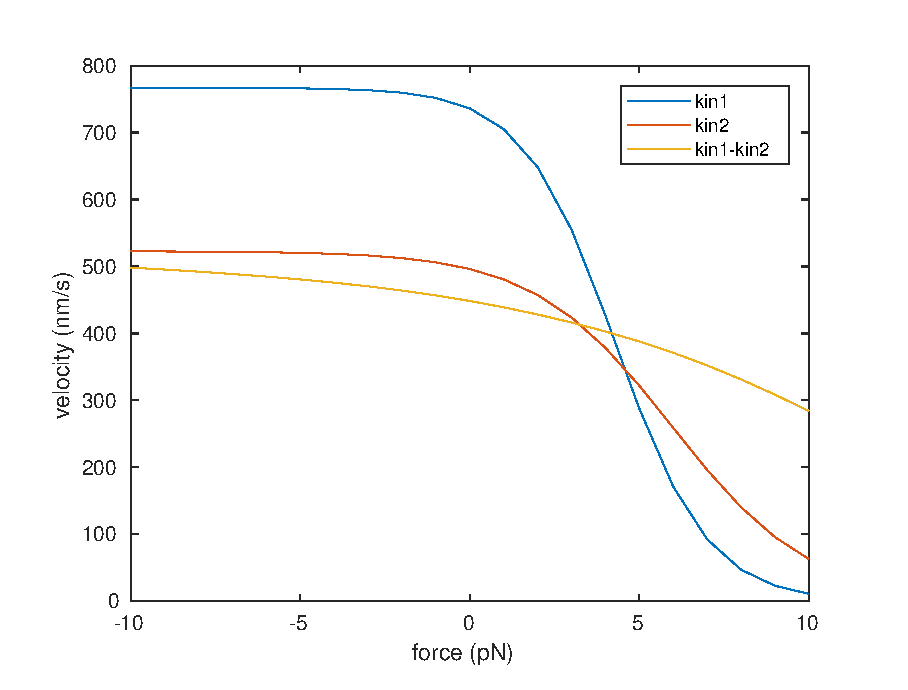
\includegraphics[scale=0.5]{figures/abc/kin1-kin2/FV}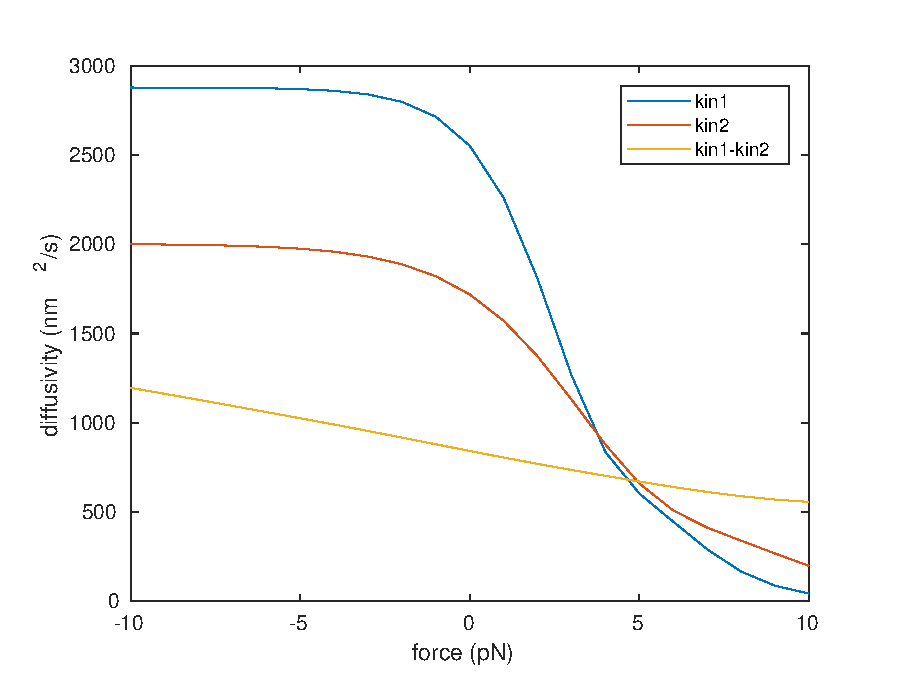
\includegraphics[scale=0.5]{figures/abc/kin1-kin2/FD}

\caption{\label{fig:stationary-distribution}Top: stationary distribution of
relative configurations of a kin1-kin1 (left) and kin1-kin2 (right)
group. Bottom: corresponding force-velocity and force-diffusivity
curves }

\end{figure}
\begin{figure}
\includegraphics[scale=0.5]{\string"figures/abc/run length/FER\string".pdf}

\caption{\label{fig:force-run-length}force-run length curves at $d_{det}=30,50,70$}

\end{figure}
\begin{table}
\begin{tabular}{|c|c|c|}
\hline 
parameter & description & value\tabularnewline
\hline 
\hline 
$k_{ab}$ & transition rate from $A$ to $B$ & 500/5000\tabularnewline
\hline 
$k_{ba}$ & transition rate from $B$ to $A$ & $0.2k_{ba}$\tabularnewline
\hline 
$k_{bc0}$ & transition rate from $B$ to $C$ under zero force & 1000\tabularnewline
\hline 
$k_{ca}$ & transition rate from $C$ to $A$ & $k_{ab}/(0.0077k_{ab}-1)$\tabularnewline
\hline 
$k_{det}$ & transition rate from $B$ to $E$ under zero force (detachment rate) & 5\tabularnewline
\hline 
$k_{att}$ & transition rate from $E$ to $A$ (attachment rate) & 50\tabularnewline
\hline 
$\delta$ & characteristic distance for $k_{bc}$ & 1\tabularnewline
\hline 
$\delta_{3},\delta_{4}$ & characteristic distance for detachment under hindering/assisting load & 0.3\tabularnewline
\hline 
\end{tabular}

\caption{\label{tab:parameters}parameters values. }
\end{table}

\subsection{cyclic 4-state model}

We use the quasi-stationary approximation in our semi-Markov approach
to study a group of 5 motors. Here what we did is a proof of concept
since biological evidence that supports quasi stationary requirements
is yet to be identified. Nevertheless, transitions $A\to F$, $A\to E$,
$F\to A$ and $F\to E$ are assumed to be force-dependent. We adopted
parameters and adapted a revised Bell's law so that the these transition
rates are at least one magnitude smaller than others to ensure validity
of quasi-stationary approximation. In Fig \ref{fig:qss-FVFD}, force-velocity
and force-diffusivity curves of the 5-motor group generated by qss1
and qss2 are shown with a comparison to MC simulation. We see that
in general qss approximation tends to overestimate velocity. But nevertheless
captured the general trend. The mismatch tend to be smaller for big
loading force which is not a surprise since it reduces the detachment
rate making the motor more quasi-stationary. With some more effort,
qss2 achieves better approximation than qss1. 

\begin{figure}
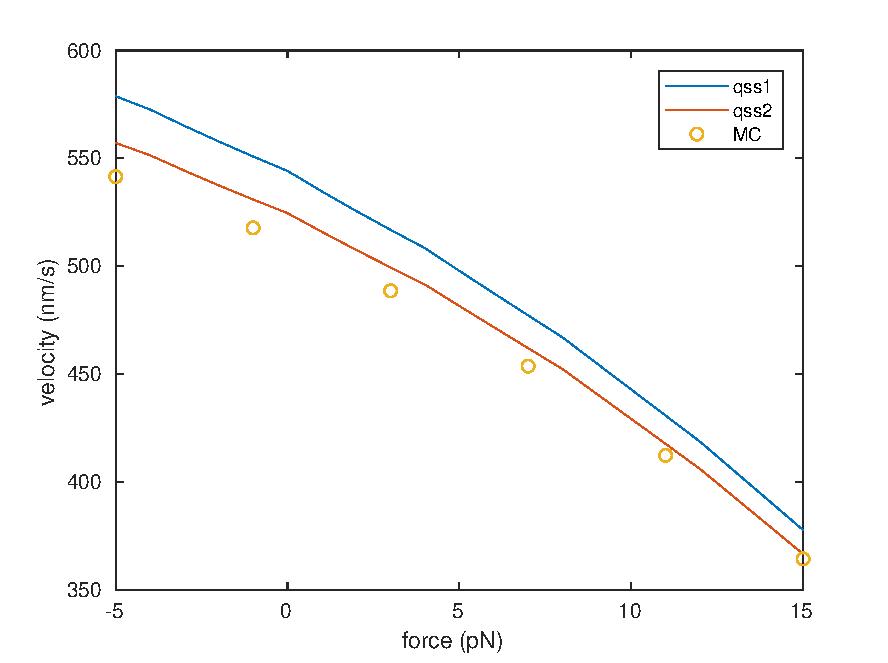
\includegraphics[scale=0.5]{figures/abcf/FVFD/FV}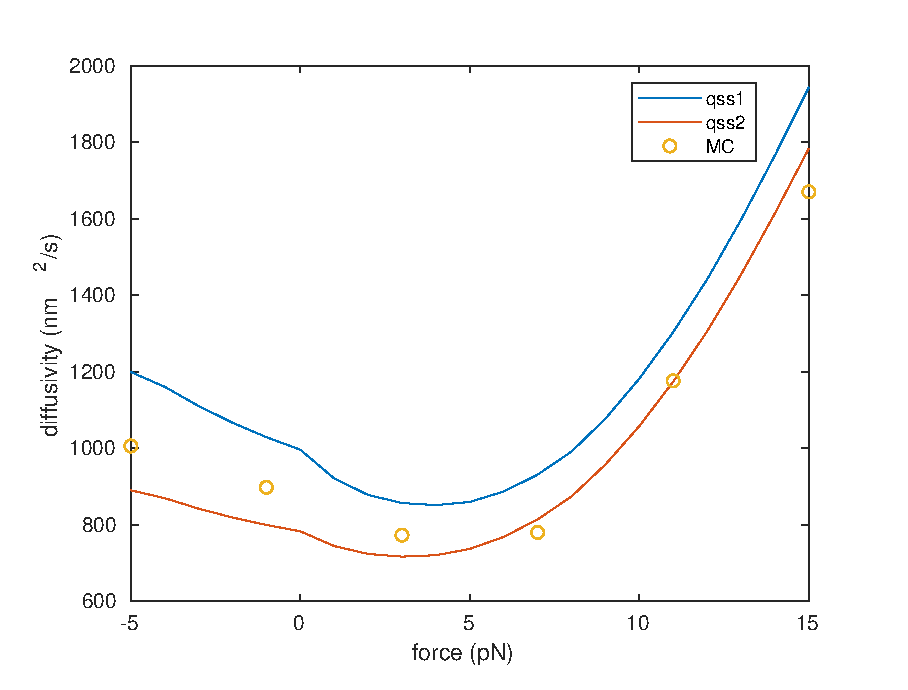
\includegraphics[scale=0.5]{figures/abcf/FVFD/FD}

\caption{\label{fig:qss-FVFD}semi-Markov with quasi-stationary approximation
(qss) compared to Monte Carlo (MC) simulation}

\end{figure}

\section{Conclusion}

In this work, we have presented a semi-Markov approach to study cellular
transportation by a group of kinesin motors. Given a kinetic model
of a single motor, we can formulate it as a semi-Markov process to
study a group of motors. By applying a functional CLT, quantities
of interests such as asymptotic velocity, diffusivity and mean run
length of the motor group can be easily calculated with a few matrix
operations. It renders much better computational efficiency than Monte
Carlo simulations without loss of underlying details of the kinetic
model. It should be noted that second moment results are usually computational
expensive using Monte Carlo simulations due to its slow convergence
with respect sample size. But it is an very important quantity to
study and plays an important role in pattern formation\cite{Brooks2016}. 

Moreover, our approach makes extensive parameter sensitivity analysis
feasible, as we demonstrated with two examples of applications. In
the first example, we applied our approach to a standard 3-state kinetic
model. We demonstrated that including detachment introduces qualitative
change into the force-velocity curve. As for diffusivity, we find
that two-motor tends to have smaller diffusivity and loading force
decreases diffusivity. Furthermore, we illustrate an example that
second-moment characteristics at single-motor level impacts the first
moment behavior in the group level: two parameter sets that have same
single-motor force-velocity response but differ in force-diffusivity
predict salient different force-velocity response of the group. We
hope that this finding will call more attention on second moments
in single molecule experiments. 

We also find that 2-motor systems tend to be slower than 1-motor system
under assisting or small hindering force while faster when under heavy
load. Hence we introduced a concept called compensation force which
is an indicator of the force regime where 2-motor system operate faster
than 1-motor system. It is of potential interests to study optimality
of cargo-motor systems. We did extensive parameter study with the
hope to spur more experimental studies on this front. 

\section{Appendix}

Here we show calculation to get $\mu_{Z},\mu_{\tau},\text{\ensuremath{\sigma_{Z},\sigma_{\tau}}}$and
$\sigma_{Z\tau}$ which are needed in (\ref{eq:V}) and (\ref{eq:D}).
To do so, we need consider a related CLT namely 
\begin{eqnarray*}
n^{1/2}\bigg(\frac{1}{n}\sum_{i=1}^{n}\begin{pmatrix}Z_{i}\\
\tau_{i}
\end{pmatrix}-\begin{pmatrix}\mu_{Z}\\
\mu_{\tau}
\end{pmatrix}\bigg) & \Rightarrow & \begin{pmatrix}U\\
T
\end{pmatrix},
\end{eqnarray*}
where the right hand side is a multivariate normal with covariance
matrix 
\[
\Sigma=\begin{pmatrix}\sigma_{Z}^{2} & \sigma_{Z\tau}\\
\sigma_{\tau Z} & \sigma_{\tau}^{2}
\end{pmatrix}.
\]
Based on assumption1, $S_{i}$ has a unique stationary distribution
$\boldsymbol{\pi}_{S}$. Based on assumption2, we know the first two
moments of $(Z_{i},\tau_{i})$ conditioned on $S_{i}$ which we denote
as $\boldsymbol{\mu}_{Z\vert S},\boldsymbol{\mu}_{\tau\vert S},\boldsymbol{\eta}_{ZZ\vert S},\boldsymbol{\eta}_{\tau\tau\vert S},\boldsymbol{\eta}_{Z\tau\vert S}$.
It is straightforward that $\mu_{Z}=\boldsymbol{\pi}_{S}'\boldsymbol{\mu}_{Z\vert S}$
and $\mu_{\tau}=\boldsymbol{\pi}_{S}'\boldsymbol{\mu}_{\tau\vert S}$.
Next we focus on the first component of $\Sigma$ for which we have
\begin{eqnarray*}
\Sigma_{11} & = & Var(Z_{i})+2\sum_{k=1}^{\infty}cov(Z_{i},Z_{i+k}).
\end{eqnarray*}
By law of total variance, we have 
\begin{eqnarray*}
Var(Z_{i}) & = & E[Var(Z_{i}\vert S_{i})]+Var(E[Z_{i}\vert S_{i}])\\
 & = & \boldsymbol{\pi}_{S}'\boldsymbol{\eta}{}_{ZZ\vert S}-\mu_{Z}^{2},
\end{eqnarray*}
where $\boldsymbol{\eta}_{ZZ\vert S}$ is the second moment of $Z$
conditioned on $S$. By law of total covariance, we have
\begin{eqnarray*}
cov(Z_{i},Z_{i+k}) & = & E[cov(Z_{i},Z_{i+k}\vert S_{i},S_{i+k})]+cov(E[Z_{i}\vert S_{i},S_{i+k}],E[Z_{i+k}\vert S_{i}, S_{i+k}]),
\end{eqnarray*}
where the first term is zero because of aussumption2 and the second
term is as follows
\begin{eqnarray*}
cov(E[Z_{i}\vert S_{i}],E[X_{i+k}\vert Z_{i+k}]) & = & (\text{\ensuremath{\boldsymbol{\mu}_{Z\vert S}}}-\mu_{Z}\boldsymbol{1})'\text{diag}(\pi_{S})P^{k}(\boldsymbol{\mu}_{Z\vert S}-\mu_{Z}\boldsymbol{1}),
\end{eqnarray*}
where $P$ is the transition matrix of the chain $\{S_{i}\}$. 

We can show that
\begin{equation}
(\text{\ensuremath{\boldsymbol{\mu}_{Z\vert S}}}-\mu_{Z}\boldsymbol{1})'\text{diag}(\boldsymbol{\pi}_{S})P^{k}(\boldsymbol{\mu}_{Z\vert S}-\mu_{Z}\boldsymbol{1})=(\text{\ensuremath{\boldsymbol{\mu}_{Z\vert S}}}-\mu_{Z}\boldsymbol{1})'\text{diag}(\boldsymbol{\pi}_{S})(P-M)^{k}(\boldsymbol{\mu}_{Z\vert S}-\mu_{Z}\boldsymbol{1}),\label{eq:(P-M)^k}
\end{equation}
 where $M$ is a $m\times m$ matrix with all entries being $1/m$.
To see this, we let $\boldsymbol{d}=\mu_{Z\vert S}-\mu_{Z}$ and $\Pi=\text{diag}(\text{\ensuremath{\pi_{S}}})$
to simplify notations. We need to use two facts: $\boldsymbol{d}'\Pi M=\boldsymbol{0}^{T}$
and $MP'=M$. We first consider $k=2$ 
\begin{eqnarray*}
\boldsymbol{d}'\Pi P^{2}\boldsymbol{d} & = & \boldsymbol{d}'\Pi(M+P-M)^{2}\boldsymbol{d}\\
 & = & \boldsymbol{d}'\Pi\big(M^{2}+M(P-M)+(P-M)M+(P-M)^{2}\big)\boldsymbol{d},
\end{eqnarray*}
where the first two terms are zero and the third term is also zero
as shown below 
\begin{eqnarray*}
\boldsymbol{d}'\Pi\big((P-M)M\big)\boldsymbol{d} & = & \boldsymbol{d}'\Pi PM\boldsymbol{d}\\
 & = & \boldsymbol{d}'M'P'\Pi'\boldsymbol{d}\\
 & = & \boldsymbol{d}'MP'\Pi\boldsymbol{d}\\
 & = & \boldsymbol{d}'M\Pi\boldsymbol{d}=0.
\end{eqnarray*}
 Thus $\boldsymbol{d}'\Pi P^{2}\boldsymbol{d}=\boldsymbol{d}'\Pi(P-M)^{2}\boldsymbol{d}.$
(\ref{eq:(P-M)^k}) follows by induction. We further note that the
spectral radius $\rho(P-M)<1$ so that $\sum_{k=0}^{\infty}(P-M)^{k}=(I-P+M)^{-1}$.
Hence 
\begin{eqnarray*}
\sum_{k=0}^{\infty}cov(Z_{i},Z_{i+k}) & = & (\text{\ensuremath{\boldsymbol{\mu}_{Z\vert S}}}-\mu_{Z}\boldsymbol{1})'\text{diag}(\boldsymbol{\pi}_{S})\big((I-P+M)^{-1}-I\big)(\boldsymbol{\mu}_{Z\vert S}-\mu_{Z}).
\end{eqnarray*}

Putting things together, we have found 
\[
\Sigma_{11}=2(\text{\ensuremath{\boldsymbol{\mu}_{Z\vert S}}}-\mu_{Z}\boldsymbol{1})'\text{diag}(\boldsymbol{\pi}_{S})(I-P+M)^{-1}(\boldsymbol{\mu}_{Z\vert S}-\mu_{Z}\boldsymbol{1})-\boldsymbol{\pi}'\boldsymbol{\eta}{}_{ZZ\vert S}+\mu_{Z}^{2}.
\]
 $\Sigma_{22}$ has the same expression for $\tau$. To find $\Sigma_{12}$,
we note that 
\[
\Sigma_{12}=cov(Z_{i},\tau_{i})+\sum_{k=1}^{\infty}cov(Z_{i},\tau_{i+k})+\sum_{k=1}^{\infty}cov(Z_{i+k},\tau_{k}).
\]
Similar calculation using law of total covariance gives 
\begin{eqnarray*}
\Sigma_{12} & = & (\text{\ensuremath{\boldsymbol{\mu}_{Z\vert S}}}-\mu_{Z}\boldsymbol{1})'\text{diag}(\boldsymbol{\pi}_{S})(I-P+M)^{-1}(\boldsymbol{\mu}_{\tau\vert S}-\mu_{\tau}\boldsymbol{1})\\
 &  & +(\text{\ensuremath{\boldsymbol{\mu}_{\tau\vert S}}}-\mu_{\tau}\boldsymbol{1})'\text{diag}(\boldsymbol{\pi}_{S})(I-P+M)^{-1}(\boldsymbol{\mu}_{Z\vert S}-\mu_{Z}\boldsymbol{1})\\
 &  & -\boldsymbol{\pi}_{S}'\boldsymbol{\eta}_{Z\tau\vert S}+\mu_{Z}\mu_{\tau}.
\end{eqnarray*}

\bibliographystyle{plain}
\bibliography{refs}

\end{document}
